\section{Rilascio}

\subsection{Come eseguire il rilascio su Windows}
Per generare l'eseguibile su Windows è necessario eseguire il file:
\newline{}\centerline{\textbf{win-dist.bat}}\newline{}
Viene generato un virtual environment di \gloman{Python} (se non presente), successivamente dopo aver installato tutte le librerie viene generato l'eseguibile all'interno della cartella \textit{dist} con il nome \textit{SSD.exe}.\\
Per leggere gli eventuali messaggi di errore, è necessario rimuovere il flag \textit{--windowed} dal file \textit{win-dist.bat}. Una volta lanciato il programma comparirà una finestra del terminale dove poter leggere gli errori presenti.
\begin{figure}[H]
    \centering
    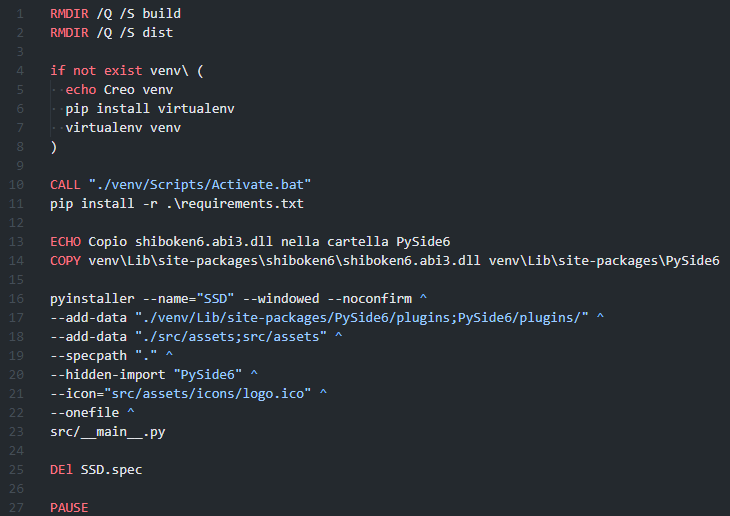
\includegraphics[scale = 0.6]{components/img/pyinstaller.png}
    \caption{File win-dist.bat}
    \label{fig:File win-dist.bat}
\end{figure}

\subsection{Come eseguire il rilascio su Linux}
Per effettuare il rilascio su Linux è necessario entrare nel virtual environment dell'ambiente di sviluppo con il comando da terminale:
\newline{}\centerline{\texttt{source venv/bin/activate}}\newline{}
in seguito bisogna dare i permessi di esecuzione ed eseguire il seguente file:
\newline{}\centerline{\texttt{chmod +x linux-dist.sh}}
\newline{}\centerline{\texttt{./linux-dist.sh}}\newline{}
Viene così creata una AppImage nella cartella \textit{dist} con il nome \textit{SSD.AppImage}. \\
Questa AppImage contiene al suo interno tutte le librerie ed il file può essere trasferito a piacimento nello stesso computer ed essere anche distribuito in altri computer con sistema operativo Linux.
\begin{figure}[H]
    \centering
    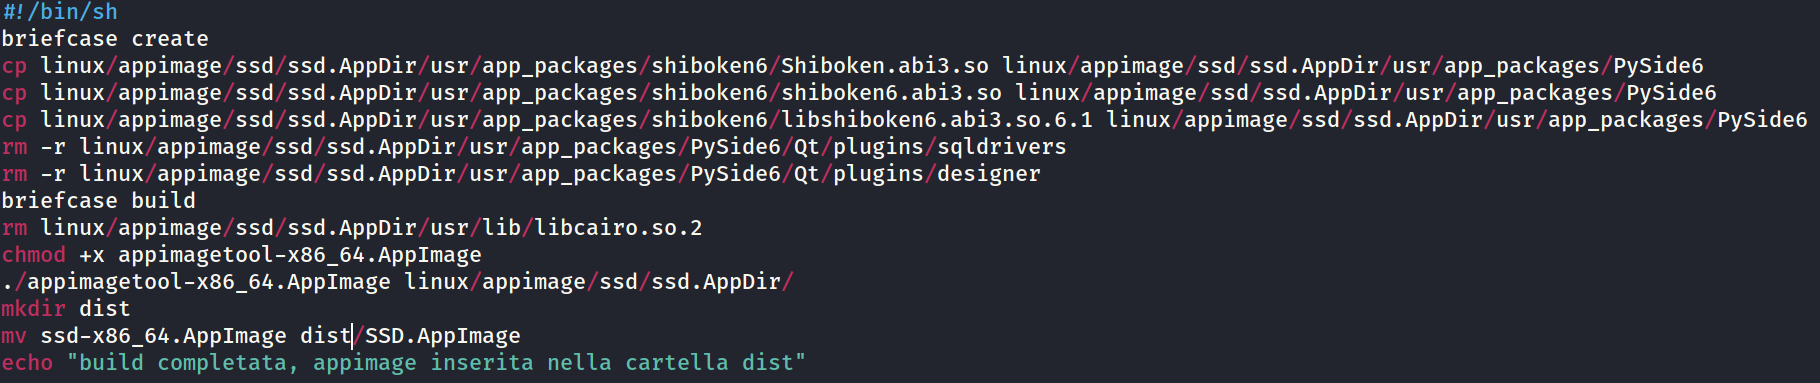
\includegraphics[scale = 0.2]{components/img/linux-deploy-script.png}
    \caption{File linux-dist.sh}
    \label{fig:File linux-dist.bat}
\end{figure}

\subsection{Come eseguire il rilascio su macOS}
Per effettuare il rilascio su macOS è necessario tramite terminale andare nella cartella di root del progetto, dare i permessi di esecuzione ed eseguire il seguente file:
\newline{}\centerline{\texttt{chmod +x mac-dist.sh}}
\newline{}\centerline{\texttt{./mac-dist.sh}}\newline{}
Viene così creato uno zip nella cartella \textit{macOS} con il nome \textit{SSD\_macOS.zip}. \\
Questo zip contiene al suo interno la AppImage e il file sh utilizzato per far partire correttamente l'applicazione.
\begin{figure}[H]
    \centering
    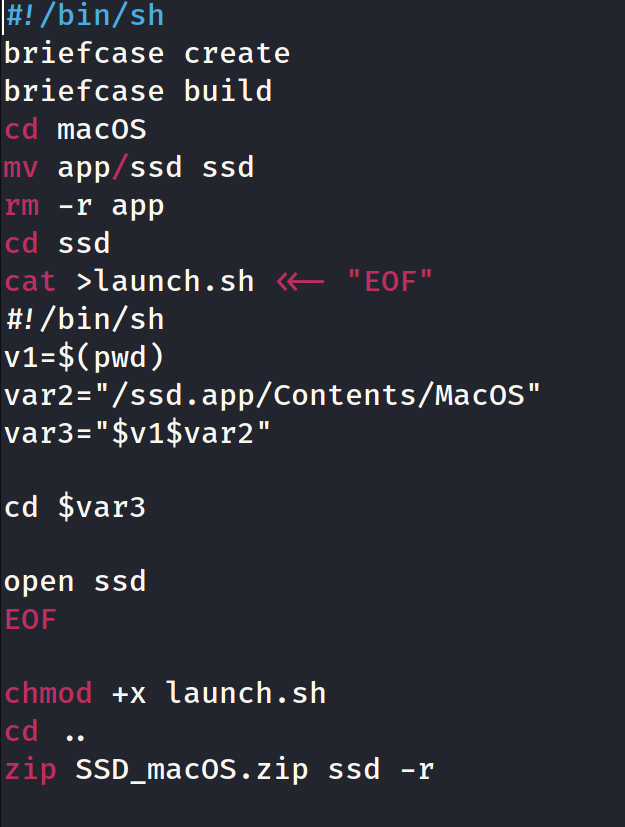
\includegraphics[scale = 0.5]{components/img/macos-deploy-script.png}
    \caption{File macos-dist.sh}
    \label{fig:File macos-dist.bat}
\end{figure}


